\section{Evaluation}
\label{sec:experiments}
\subsection{Experiment Setup}

We demonstrate our attack on two stream query benchmarks:  SecureStream \cite{DBLP:journals/corr/abs-1805-01752} and NEXMark \cite{nexmark}. Each benchmark consists of a set of representative queries, which we deployed on our system to collect processing time data for operator classification and parameter inference.

\noindent \textbf{SecureStream.} This benchmark consists of a simple map-filter-reduce pipeline designed to process a real-world dataset released by the U.S. Bureau of Transportation Statistics. The dataset contains over $14$ million flight records from multiple air carriers. We discuss the benchmark's operators in Appendix~\ref{app:benchmark}. 

\noindent \textbf{NEXMark.} This benchmark is widely used to evaluate stream processing systems~\cite{begoli2019one,hoffmann2019megaphone,sponge2023,Meces2022,three_step_2018}. It targets online auction applications. It consists of three types of data events: Person, Auction, and Bid, representing three typical entities in the auction context. We conduct our experiments using the first six queries, covering a diverse range of operator types and dataflow patterns. The last two queries are only a replication of previous ones and are therefore omitted without loss of generality. Since our system only implements basic operators with simple window mechanisms, each query is simplified if necessary and then represented as a Directed Acyclic Graph (DAG) of implemented stream operators, which defines the flow of data through the system. A summary of the deployed queries is presented in Appendix~\ref{app:benchmark}. 

\noindent{\bf Timing dataset.}  We executed the deployed queries using a mix of collected and synthetically generated data as input. We systematically vary the query parameters. For Map and Filter operators, we replaced the fixed mapping and filtering conditions in the original queries with multiple alternative expressions. For window-based operators, we altered the window size and sliding step values across runs. Table~\ref{tab:dataset} summarizes the results. 

\begin{table}
\caption{Timing dataset.}
\label{tab:dataset}
\begin{tabular}{lc|lc}
\hline
\multicolumn{2}{c|}{\textbf{SecureStream benchmark}}                            & \multicolumn{2}{c}{\textbf{NEXMark benchmark}}                       \\ \hline
\textbf{Operator}             & \multicolumn{1}{l|}{\textbf{No. of samples}} & \textbf{Operator}   & \multicolumn{1}{l}{\textbf{No. of samples}} \\ \hline
Map                           & 350                                             & Map                 & 1262                                           \\
Filter                        & 350                                             & Filter              & 1297                                           \\
Reduce                        & 350                                             & Join                & 1009                                           \\
\multicolumn{1}{c}{\textbf{}} & \multicolumn{1}{l|}{}                           & Max                 & 1059                                           \\
                              &                                                 & Average   & 1018                                           \\
                              &                                                 & Avg (Partition) & 1071                                           \\ \hline
\textit{Total}                & 1050                                            & \textit{Total}      & 6716                                           \\ \hline
\end{tabular}
\end{table}


\subsubsection*{Hardware specifications}
Experiments are conducted on a computer running Ubuntu 22.04 equipped with Intel(R) Core(TM) i5-9300H, 4 physical cores, and 16 GB RAM, with SGX version I.

\subsection{Results}
\label{subsec:results}

\begin{figure*}
    \centering
    \begin{subfigure}[t]{0.3\textwidth}
        \includegraphics[width=0.9\linewidth]{Figures/NEXMark_cdf_Q1_Map.pdf}
        \caption{Map}
    \end{subfigure}%
    \hfill
    \begin{subfigure}[t]{0.3\textwidth}
        \includegraphics[width=0.9\linewidth]{Figures/NEXMark_cdf_Q2_Filter.pdf}
        \caption{Filter}
    \end{subfigure}%
    \hfill
    \begin{subfigure}[t]{0.3\textwidth}
        \includegraphics[width=0.9\linewidth]{Figures/NEXMark_cdf_Q3_Join.pdf}
        \caption{Join}
    \end{subfigure}%

    \vspace{1mm}
    \begin{subfigure}[t]{0.3\textwidth}
        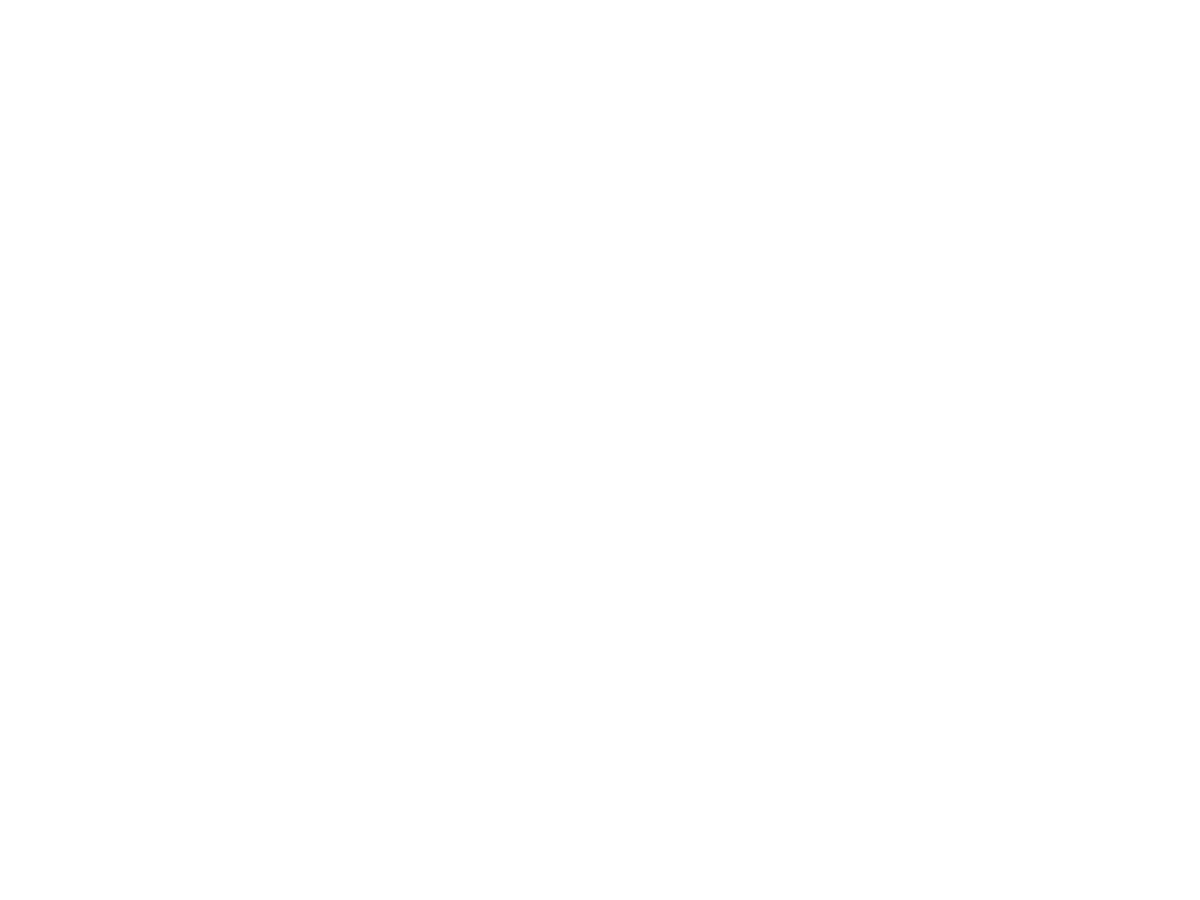
\includegraphics[width=0.9\linewidth]{Figures/nexmark_cdf_Q6_Avg_Partition.pdf}
        \caption{Average (Partition)}
    \end{subfigure}%
    \hfill
    \begin{subfigure}[t]{0.3\textwidth}
        \includegraphics[width=0.9\linewidth]{Figures/NEXMark_cdf_Q5_Count_Auction.pdf}
        \caption{Count}
    \end{subfigure}%
    \hfill
    \begin{subfigure}[t]{0.3\textwidth}
        \includegraphics[width=0.9\linewidth]{Figures/NEXMark_cdf_Q4_Max.pdf}
        \caption{Max}
    \end{subfigure}%
    \caption{CDFs of operators' timing distributions.}
    \label{fig:cdf_of_each_operators}
\end{figure*}

\subsubsection{CDF-based representation} Figure~\ref{fig:cdf_of_each_operators} illustrates representative CDF curves for six operator types: Map, Filter, Join, Average, Count, and Max. The x-axis (\textit{Time}) represents the measured RDTSCP values, while the y-axis corresponds to the computed cumulative probability.

The Map operator (see Figure \ref{fig:cdf_of_each_operators}.a) exhibits a smooth, continuous CDF curve. This is expected, as Map applies a simple, stateless transformation uniformly to all incoming events, leading to consistent processing durations with minimal variance.

In contrast, the CDF for the Filter operator (see Figure \ref{fig:cdf_of_each_operators}.b) displays a noticeable “leap” or abrupt increase in the slope around the midpoint. This discontinuity reflects the operator's branching behavior: input events that satisfy the filtering condition are passed downstream, typically incurring a slightly longer processing time, while events that are filtered out are processed more quickly. This dichotomy results in two dominant processing time modes and causes the CDF to exhibit a step-like feature.

A similar pattern is observed in the Join operator (see Figure \ref{fig:cdf_of_each_operators}.c), but with some key differences. 
%
The leap in the Join CDF occurs at a different location along the x-axis, and the gap between the two processing modes is more pronounced. 
%
This is due to the nature of stream joins, which depend on the window state. When a new event arrives but the corresponding join window is incomplete or has not yet slid forward sufficiently, the operator performs only state maintenance, leading to shorter execution times. When the window becomes complete, the join computation is triggered, resulting in a significant increase in processing time—hence the sharper and wider leap in the CDF.

The final group—Average, Count, and Max—share a common structure, as they are all windowed aggregation operators (see Figures \ref{fig:cdf_of_each_operators}.d-f). 
%
Their CDFs exhibit similar leap patterns, akin to the Join operator, due to the windowing behavior. 
%
While the precise computation differs (e.g., summing for average vs. scanning for maximum), the general processing pattern remains consistent: periods of lightweight state updates punctuated by more expensive aggregation computations when the window criteria are satisfied.

These observations demonstrate that CDF curves can effectively capture structural differences in operator behavior, offering a visually intuitive and statistically meaningful representation for operator classification.

\subsubsection{TS2Vec-based representation} The TS2Vec model was trained on the timing dataset for 10 epochs, with an output embedding dimension of 1024. 
%
Figure~\ref{fig:ts2vec-tsne} presents the resulting 2D projection of the embeddings using t-distributed Stochastic Neighbor Embedding (t-SNE). Each point corresponds to a time series representation of an operator execution, colored according to its operator type. The figure reveals that, in general, embeddings from different operators form distinguishable clusters, indicating that TS2Vec is effective in capturing operator-specific temporal patterns for classification purposes.

However, we also observe that samples from the Filter operator exhibit substantial overlap with those from the Map operator. This suggests that, in practice, distinguishing between these two stateless operators based on timing behavior alone may be challenging. The similarity in processing logic—both operators apply a single-event transformation without maintaining state—likely contributes to this ambiguity in the latent space.

\begin{figure}
    \centering
        \includegraphics[width=0.8\linewidth]{Figures/NEXMark_tsne_plot.pdf}
    \caption{t-SNE visualization of NEXMark TS2Vec embeddings}
    \label{fig:ts2vec-tsne}
\end{figure}

\subsubsection{Operator classification on single benchmark} We evaluate the effectiveness of three widely used machine learning models—Random Forest (RF), Support Vector Machine (SVM), and XGBoost—for operator classification based on timing representations. For each model, we perform a grid search over various combinations of hyperparameters (refer to Appendix~\ref{app:evalution}), and use 5-fold cross-validation to ensure robustness and reduce overfitting. Table \ref{tab:performances_single_benchmark} reports the best classification accuracy achieved by each model under both CDF-based and TS2Vec-based representations.


\begin{table*}
\centering
\caption{Performance of operator classification models}
\label{tab:performances_single_benchmark}
\begin{tabular}{lcccccccc}
\hline
\multicolumn{1}{c}{\multirow{2}{*}{\textbf{Models}}} & \multicolumn{4}{c}{\textbf{SecureStream benchmark}}                                                                      & \multicolumn{4}{c}{\textbf{NEXMark benchmark}}                                                                           \\ \cline{2-9} 
\multicolumn{1}{c}{}                                 & \multicolumn{1}{l}{Accuracy} & \multicolumn{1}{l}{Precision} & \multicolumn{1}{l}{Recall} & \multicolumn{1}{l}{F1 score} & \multicolumn{1}{l}{Accuracy} & \multicolumn{1}{l}{Precision} & \multicolumn{1}{l}{Recall} & \multicolumn{1}{l}{F1 score} \\ \hline
\multicolumn{9}{c}{\textbf{CDF}}                                                                                                                                                                                                                                                                           \\ \hline
Random Forest                                        & 0.8503                       & 0.8399                        & 0.8316                     & 0.8311                       & 0.7178                       & 0.7757                        & 0.7440                     & 0.7262                       \\
SVM                                                  & 0.8503                       & 0.8413                        & 0.8314                     & 0.8310                       & 0.7735                       & 0.8005                        & 0.7979                     & 0.7791                       \\
XGBoost                                              & 0.8569                       & 0.8502                        & 0.8384                     & 0.8378                       & 0.6637                       & 0.6834                        & 0.7093                     & 0.6179                       \\ \hline
\multicolumn{9}{c}{\textbf{TS2Vec Embedding}}                                                                                                                                                                                                                                                              \\ \hline
Random Forest                                        & 0.8914                       & 0.9077                        & 0.8758                     & 0.8748                       & 0.8479                       & 0.8798                        & 0.8733                     & 0.8635                       \\
SVM                                                  & 0.9145                       & 0.9072                        & 0.9047                     & 0.9052                       & \textbf{0.8662}                       & \textbf{0.8916}                        & \textbf{0.8894}                     & \textbf{0.8853}                       \\
XGBoost                                              & \textbf{0.9211}                       & \textbf{0.9253}                        & \textbf{0.9102}                     & \textbf{0.9110}                       & 0.8510                       & 0.8915                        & 0.8805                     & 0.8684                       \\ \hline
\end{tabular}
\end{table*}

Overall, models trained on TS2Vec embeddings consistently outperform those trained on CDF features. On the SecureStream benchmark, all three models achieve comparable performance with CDF features, yielding approximately 85\% accuracy. When switching to TS2Vec embeddings, classification accuracy improves for all models. XGBoost achieves the highest accuracy of 92\%, representing a 7\% improvement over its CDF-based counterpart and a 1--2\% margin over the other TS2Vec-based models.

A similar trend is observed on the NEXMark benchmark. Under CDF features, none of the models surpass 80\% accuracy; notably, XGBoost performs the worst, achieving only 66\%. In contrast, using TS2Vec embeddings boosts the accuracy of all three models by at least 10\%. SVM emerges as the top-performing model on this benchmark, achieving 86\% accuracy—1--2\% higher than both Random Forest and XGBoost.

These results demonstrate that TS2Vec is a more effective feature representation for operator classification tasks, particularly in capturing the temporal structure present in timing data.

%It is worth noting that the best-performing model varies across benchmarks. For example, XGBoost performs best on SecureStream, while SVM achieves the highest accuracy on NEXMark. This inconsistency highlights a challenge for attackers: it is difficult to design a single classification model that generalizes well across different data processing environments. As a result, attacks relying on operator classification may require benchmark-specific tuning to maintain effectiveness.

\subsubsection{Confusion matrix} The confusion matrix of the best-performing TS2Vec-based models for NEXMark is presented in Figure \ref{fig:confusion_matrix_nexmark} (we discuss both benchmarks in more detail in Appendix~\ref{app:evalution}). We observe that the model misclassifies 64\% of Map samples and 17\% of Filter samples as the other class. Additionally, the model struggles to differentiate between the Max and Average (sliding) operators. This can be attributed to their shared characteristics as aggregation functions operating over sliding windows. 
%Interestingly, the Count operator—despite also being an aggregation function with the same windowing mechanism—is classified more accurately. This could be because it performs simpler logic (i.e., incrementing a count) without the need for value comparisons or numerical calculations, making its timing behavior more consistent and distinguishable.


\begin{figure}
    \centering
    \begin{subfigure}[t]{0.45\textwidth}
        \includegraphics[width=\linewidth]{Figures/svr_NEXMark_ts2vec_confusion_matrix.pdf}
    \end{subfigure}
    \caption{Confusion matrix (NEXMark)} % of the best models of each benchmark}
    \label{fig:confusion_matrix_nexmark}
\end{figure}


\subsubsection{Cross-benchmark operator classification} To evaluate the generalizability of operator classification models across benchmarks, we retrained the best-performing model from the NEXMark benchmark on its entire dataset and tested its performance on the SecureStream benchmark. The \textit{Reduce} operator in SecureStream can be considered as the \textit{Average (Sliding)} operator in the NEXMark benchmark. The results, summarized in Table \ref{tab:cross_performances}, reveal a significant drop in performance when models are applied outside of their training domain.

As expected, no models achieved an accuracy above 80\% in this cross-benchmark setting. Interestingly, the best result was obtained by the CDF-based XGBoost model, which achieved 80\% accuracy, 79\% precision, 78\% recall, and a 78\% F1-score. In contrast, TS2Vec-based models, which had outperformed their CDF counterparts in within-benchmark evaluations, showed poor generalization: all TS2Vec-based models failed to surpass 50\% on any metric.

These findings indicate a trade-off between specificity and generalizability. TS2Vec embeddings are highly effective when trained and tested on the same benchmark, likely due to their capacity to learn benchmark-specific temporal patterns. On the other hand, the CDF representation, though less effective for within-benchmark classification, appears to offer greater robustness and transferability across benchmarks.

\begin{table}
\centering
\caption{Performance of NEXMark models on SecureStream benchmark}
\label{tab:cross_performances}
\begin{tabular}{lcccc}
\hline
\multicolumn{1}{c}{\multirow{2}{*}{\textbf{Models}}} & \multicolumn{4}{c}{\textbf{Metrics}}                                                                                     \\ \cline{2-5} 
\multicolumn{1}{c}{}                                 & \multicolumn{1}{l}{Accuracy} & \multicolumn{1}{l}{Precision} & \multicolumn{1}{l}{Recall} & \multicolumn{1}{l}{F1 score} \\ \hline
\multicolumn{5}{c}{\textbf{CDF}}                                                                                                                                                \\ \hline
Random Forest                                        & 0.6140                       & 0.7681                        & 0.6190                     & 0.6460                       \\
SVM                                                  & 0.7169                       & 0.7632                        & 0.7057                     & 0.7186                       \\
\textbf{XGBoost}                                              & \textbf{0.8008}                       & \textbf{0.7935}                        & \textbf{0.7842}                     & \textbf{0.7819}                       \\ \hline
\multicolumn{5}{c}{\textbf{TS2Vec Embedding}}                                                                                                                                   \\ \hline
Random Forest                                        & 0.4864                       & 0.5108                        & 0.5031                     & 0.5034                       \\
SVM                                                  & 0.4255                       & 0.4324                        & 0.4246                     & 0.4165                       \\
XGBoost                                              & 0.4790                       & 0.4751                        & 0.4751                     & 0.4751                       \\ \hline
\end{tabular}
\end{table}

\subsubsection{Query recovery}
We now evaluate the success rate of recovering the entire query, as opposed to recovering individual operators. This is an important metric because a query comprises multiple distinct operators, the attacker must identify all the operators in order to learn the query. Even when one operator is recovered with high accuracy (e.g., 92\%), it does not necessarily follow that the query can be recovered with the same level of accuracy. We use Query Recovery Successful Rate (QRSR) metric, which quantifies the degree to which a query can be reconstructed. QRSR is defined as the product of the classification accuracies of all the operators in the query.

We train and evaluate the models under two settings. In the first setting, operators from all queries are divided evenly into training and testing sets. Each model is trained on the training subset and evaluated on the testing subset. In the second setting, all operators belonging to one query are withheld for testing, while operators from the remaining queries are used for training. Experiments under this setting are repeated with a different query withheld each time. We only consider the NEXMark benchmark, since the SecureStream benchmark includes only a single query consisting of three operators.

\begin{table*}
\centering
\scriptsize
\caption{Query Recovery Success Rate (QRSR) in the first setting}
\label{tab:qrsr_first_setting}
\begin{tabular}{cccccclccclccc}
\hline
\multirow{2}{*}{\textbf{Query}} & \multirow{2}{*}{\textbf{Operators}} & \multirow{2}{*}{\textbf{\begin{tabular}[c]{@{}c@{}}No. \\Samples\end{tabular}}} & \multicolumn{3}{c}{\textbf{Random Forest}}                                                                                                                                           &                      & \multicolumn{3}{c}{\textbf{SVM}}                                                                                                                                                     &                      & \multicolumn{3}{c}{\textbf{XGBoost}}                                                                                                                                                     \\ \cline{4-6} \cline{8-10} \cline{12-14} 
                                &                                     &                                       & \textbf{\begin{tabular}[c]{@{}c@{}}Correctly\\ Predicted\end{tabular}} & \textbf{\begin{tabular}[c]{@{}c@{}}\% Correctly\\ Predicted\end{tabular}} & \textbf{QRSR}                   &                      & \textbf{\begin{tabular}[c]{@{}c@{}}Correctly\\ Predicted\end{tabular}} & \textbf{\begin{tabular}[c]{@{}c@{}}\% Correctly\\ Predicted\end{tabular}} & \textbf{QRSR}                   &                      & \textbf{\begin{tabular}[c]{@{}c@{}}Correctly\\ Predicted\end{tabular}} & \textbf{\begin{tabular}[c]{@{}c@{}}\% Correctly\\ Predicted\end{tabular}} & \textbf{QRSR}                   \\ \hline
\multicolumn{14}{c}{\textbf{CDF}}                                                                                                                                                                                                                                                                                                                                                                                                                                                                                                                                                                                                                                                                                                \\ \hline
Q1                              & Map                                 & 123                                   & 118                                                                    & 95.93                                                                     & \textbf{95.93}                  &                      & 108                                                                    & 87.80                                                                     & \textbf{87.80}                  &                      & 118                                                                    & 95.93                                                                     & \textbf{95.93}                  \\ \hline
\multirow{2}{*}{Q2}             & Filter                              & 152                                   & 135                                                                    & 88.82                                                                     & \multirow{2}{*}{\textbf{88.82}} &                      & 110                                                                    & 72.37                                                                     & \multirow{2}{*}{\textbf{70.63}} &                      & 123                                                                    & 80.92                                                                     & \multirow{2}{*}{\textbf{80.92}} \\
                                & Map                                 & 125                                   & 125                                                                    & 100                                                                       &                                 &                      & 122                                                                    & 97.6                                                                      &                                 &                      & 125                                                                    & 100                                                                       &                                 \\ \hline
\multirow{4}{*}{Q3}             & Filter 1                            & 186                                   & 185                                                                    & 99.46                                                                     & \multirow{4}{*}{\textbf{97.26}} &                      & 172                                                                    & 92.47                                                                     & \multirow{4}{*}{\textbf{49.81}} &                      & 185                                                                    & 99.46                                                                     & \multirow{4}{*}{\textbf{97.77}} \\
                                & Filter 2                            & 150                                   & 149                                                                    & 99.33                                                                     &                                 &                      & 142                                                                    & 94.67                                                                     &                                 &                      & 149                                                                    & 99.33                                                                     &                                 \\
                                & Join                                & 252                                   & 252                                                                    & 100                                                                       &                                 &                      & 148                                                                    & 58.73                                                                     &                                 &                      & 252                                                                    & 100                                                                       &                                 \\
                                & Map                                 & 192                                   & 189                                                                    & 98.44                                                                     &                                 &                      & 186                                                                    & 96.88                                                                     &                                 &                      & 190                                                                    & 98.96                                                                     &                                 \\ \hline
\multirow{4}{*}{Q4}             & Join                                & 253                                   & 253                                                                    & 100                                                                       & \multirow{4}{*}{\textbf{97.53}} &                      & 249                                                                    & 98.42                                                                     & \multirow{4}{*}{\textbf{90.00}} &                      & 251                                                                    & 99.21                                                                     & \multirow{4}{*}{\textbf{86.47}} \\
                                & Map                                 & 192                                   & 188                                                                    & 97.92                                                                     &                                 &                      & 178                                                                    & 92.71                                                                     &                                 &                      & 168                                                                    & 87.5                                                                      &                                 \\
                                & Max                                 & 256                                   & 256                                                                    & 100                                                                       &                                 &                      & 253                                                                    & 98.83                                                                     &                                 &                      & 256                                                                    & 100                                                                       &                                 \\
                                & Average                             & 509                                   & 507                                                                    & 99.61                                                                     &                                 &                      & 508                                                                    & 99.80                                                                     &                                 &                      & 507                                                                    & 99.61                                                                     &                                 \\ \hline
Q5                              & Count                               & 375                                   & 375                                                                    & 100                                                                       & \textbf{100}                    &                      & 372                                                                    & 99.2                                                                      & \textbf{99.2}                   &                      & 375                                                                    & 100                                                                       & \textbf{100}                    \\ \hline
\multirow{3}{*}{Q6}             & Filter                              & 161                                   & 136                                                                    & 84.47                                                                     & \multirow{3}{*}{\textbf{84.47}} &                      & 138                                                                    & 85.71                                                                     & \multirow{3}{*}{\textbf{84.59}} &                      & 121                                                                    & 75.16                                                                     & \multirow{3}{*}{\textbf{75.02}} \\
                                & Max                                 & 547                                   & 547                                                                    & 100                                                                       &                                 &                      & 547                                                                    & 100                                                                       &                                 &                      & 546                                                                    & 99.82                                                                     &                                 \\
                                & Average (P)                         & 536                                   & 536                                                                    & 100                                                                       &                                 &                      & 529                                                                    & 98.69                                                                     &                                 &                      & 536                                                                    & 100                                                                       &                                 \\ \hline
\multicolumn{14}{c}{\textbf{TS2Vec Embedding}}                                                                                                                                                                                                                                                                                                                                                                                                                                                                                                                                                                                                                                                                                   \\ \hline
Q1                              & Map                                 & 123                                   & 119                                                                    & 96.75                                                                     & \textbf{96.75}                  &                      & 113                                                                    & 91.87                                                                     & \textbf{91.87}                  &                      & 116                                                                    & 94.31                                                                     & \textbf{94.31}                  \\ \hline
\multirow{2}{*}{Q2}             & Filter                              & 152                                   & 121                                                                    & 79.61                                                                     & \multirow{2}{*}{\textbf{78.33}} &                      & 122                                                                    & 80.26                                                                     & \multirow{2}{*}{\textbf{76.41}} &                      & 120                                                                    & 78.94                                                                     & \multirow{2}{*}{\textbf{78.32}} \\
                                & Map                                 & 125                                   & 123                                                                    & 98.40                                                                     &                                 & \multicolumn{1}{c}{} & 119                                                                    & 95.20                                                                     &                                 & \multicolumn{1}{c}{} & 124                                                                    & 99.2                                                                      &                                 \\ \hline
\multirow{4}{*}{Q3}             & Filter 1                            & 186                                   & 136                                                                    & 73.12                                                                     & \multirow{4}{*}{\textbf{63.88}} &                      & 152                                                                    & 81.72                                                                     & \multirow{4}{*}{\textbf{66.28}} &                      & 143                                                                    & 76.88                                                                     & \multirow{4}{*}{\textbf{64.47}} \\
                                & Filter 2                            & 150                                   & 136                                                                    & 90.67                                                                     &                                 & \multicolumn{1}{c}{} & 138                                                                    & 92.00                                                                     &                                 & \multicolumn{1}{c}{} & 136                                                                    & 90.67                                                                     &                                 \\
                                & Join                                & 252                                   & 252                                                                    & 100                                                                       &                                 & \multicolumn{1}{c}{} & 248                                                                    & 98.41                                                                     &                                 & \multicolumn{1}{c}{} & 250                                                                    & 99.21                                                                     &                                 \\
                                & Map                                 & 192                                   & 185                                                                    & 96.35                                                                     &                                 & \multicolumn{1}{c}{} & 172                                                                    & 89.58                                                                     &                                 & \multicolumn{1}{c}{} & 179                                                                    & 93.23                                                                     &                                 \\ \hline
\multirow{4}{*}{Q4}             & Join                                & 253                                   & 253                                                                    & 100                                                                       & \multirow{4}{*}{\textbf{85.03}} &                      & 252                                                                    & 99.60                                                                     & \multirow{4}{*}{\textbf{80.69}} &                      & 253                                                                    & 100                                                                       & \multirow{4}{*}{\textbf{82.80}} \\
                                & Map                                 & 192                                   & 188                                                                    & 97.92                                                                     &                                 & \multicolumn{1}{c}{} & 178                                                                    & 92.71                                                                     &                                 & \multicolumn{1}{c}{} & 184                                                                    & 95.83                                                                     &                                 \\
                                & Max                                 & 256                                   & 256                                                                    & 100                                                                       &                                 & \multicolumn{1}{c}{} & 247                                                                    & 96.48                                                                     &                                 & \multicolumn{1}{c}{} & 253                                                                    & 98.828125                                                                 &                                 \\
                                & Average                             & 509                                   & 442                                                                    & 86.84                                                                     &                                 & \multicolumn{1}{c}{} & 461                                                                    & 90.57                                                                     &                                 & \multicolumn{1}{c}{} & 445                                                                    & 87.43                                                                     &                                 \\ \hline
Q5                              & Count                               & 375                                   & 374                                                                    & 99.73                                                                     & \textbf{99.73}                  &                      & 374                                                                    & 99.73                                                                     & \textbf{99.73}                  &                      & 374                                                                    & 99.73                                                                     & \textbf{99.73}                  \\ \hline
\multirow{3}{*}{Q6}             & Filter                              & 161                                   & 119                                                                    & 73.91                                                                     & \multirow{3}{*}{\textbf{73.51}} &                      & 132                                                                    & 81.99                                                                     & \multirow{3}{*}{\textbf{79.29}} &                      & 121                                                                    & 75.16                                                                     & \multirow{3}{*}{\textbf{74.04}} \\
                                & Max                                 & 547                                   & 545                                                                    & 99.63                                                                     &                                 &                      & 534                                                                    & 97.62                                                                     &                                 &                      & 543                                                                    & 99.27                                                                     &                                 \\
                                & Average (P)                         & 536                                   & 535                                                                    & 99.81                                                                     &                                 &                      & 531                                                                    & 99.07                                                                     &                                 &                      & 532                                                                    & 99.25                                                                     &                                 \\ \hline
\end{tabular}
\end{table*}

Table \ref{tab:qrsr_first_setting} shows the results under the first setting. Using CDF, all models achieved a QRSR of at least 80\% across all queries, except for the XGBoost model on Query 6 (Q6). Among the tested models, Random Forest consistently outperformed others, demonstrating dominant performance in nearly all cases. Notably, using CDF results in a high QRSR even in complex queries such as Q3 and Q4, both of which involve multiple operators. TS2Vec leads to poorer performance. In particular, three out of six queries have QRSR values below 80\%. These findings diverge from the results reported earlier in Table \ref{tab:performances_single_benchmark}, where TS2Vec outperforms CDF.

\begin{table*}
\centering
\scriptsize
\caption{Query Recovery Success Rate (QRSR) in the second setting}
\label{tab:qrsr_second_setting}
\begin{tabular}{cccccccccccccc}
\hline
\multirow{2}{*}{\textbf{Query}} & \multirow{2}{*}{\textbf{Operators}} & \multirow{2}{*}{\textbf{\begin{tabular}[c]{@{}c@{}}No. \\Samples\end{tabular}}} & \multicolumn{3}{c}{\textbf{Random Forest}}                                                                                                                                             & \textbf{} & \multicolumn{3}{c}{\textbf{SVM}}                                                                                                                                                       & \textbf{} & \multicolumn{3}{c}{\textbf{XGBoost}}                                                                                                                                                       \\ \cline{4-6} \cline{8-10} \cline{12-14} 
                                &                                     &                                 & \textbf{\begin{tabular}[c]{@{}c@{}}Correctly\\ Classified\end{tabular}} & \textbf{\begin{tabular}[c]{@{}c@{}}\% Correctly\\ Classified\end{tabular}} & \textbf{QRSR}                   & \textbf{} & \textbf{\begin{tabular}[c]{@{}c@{}}Correctly\\ Classified\end{tabular}} & \textbf{\begin{tabular}[c]{@{}c@{}}\% Correctly\\ Classified\end{tabular}} & \textbf{QRSR}                   & \textbf{} & \textbf{\begin{tabular}[c]{@{}c@{}}Correctly\\ Classified\end{tabular}} & \textbf{\begin{tabular}[c]{@{}c@{}}\% Correctly\\ Classified\end{tabular}} & \textbf{QRSR}                   \\ \hline
\multicolumn{14}{c}{CDF}                                                                                                                                                                                                                                                                                                                                                                                                                                                                                                                                                                                                                                                                                   \\ \hline
Q1                              & Map                                 & 245                             & 144                                                                     & 58.78                                                                      & \textbf{58.78}                  &           & 211                                                                     & 86.12                                                                      & \textbf{86.12}                  &           & 118                                                                     & 48.16                                                                      & \textbf{48.16}                  \\ \hline
\multirow{2}{*}{Q2}             & Filter                              & 304                             & 211                                                                     & 69.41                                                                      & \multirow{2}{*}{\textbf{69.41}} &           & 167                                                                     & 54.93                                                                      & \multirow{2}{*}{\textbf{53.61}} &           & 146                                                                     & 48.03                                                                      & \multirow{2}{*}{\textbf{48.03}} \\
                                & Map                                 & 249                             & 249                                                                     & 100                                                                        &                                 &           & 243                                                                     & 97.59                                                                      &                                 &           & 249                                                                     & 100                                                                        &                                 \\ \hline
\multirow{4}{*}{Q3}             & Filter 1                            & 372                             & 347                                                                     & 93.28                                                                      & \multirow{4}{*}{\textbf{0.09}}  &           & 234                                                                     & 62.90                                                                      & \multirow{4}{*}{\textbf{0.99}}  &           & 259                                                                     & 69.62                                                                      & \multirow{4}{*}{\textbf{0.29}}  \\
                                & Filter 2                            & 300                             & 207                                                                     & 69.00                                                                      &                                 &           & 131                                                                     & 43.67                                                                      &                                 &           & 103                                                                     & 34.33                                                                      &                                 \\
                                & Join                                & 504                             & 10                                                                      & 1.98                                                                       &                                 &           & 38                                                                      & 7.54                                                                       &                                 &           & 15                                                                      & 2.98                                                                       &                                 \\
                                & Map                                 & 384                             & 28                                                                      & 7.29                                                                       &                                 &           & 183                                                                     & 47.66                                                                      &                                 &           & 158                                                                     & 41.15                                                                      &                                 \\ \hline
\multirow{3}{*}{Q4}             & Join                                & 505                             & 251                                                                     & 49.70                                                                      & \multirow{3}{*}{\textbf{4.24}}  &           & 217                                                                     & 42.97                                                                      & \multirow{3}{*}{\textbf{22.14}} &           & 10                                                                      & 1.98                                                                       & \multirow{3}{*}{\textbf{0}}     \\
                                & Map                                 & 384                             & 40                                                                      & 10.42                                                                      &                                 &           & 287                                                                     & 74.74                                                                      &                                 &           & 0                                                                       & 0                                                                          &                                 \\
                                & Max                                 & 512                             & 419                                                                     & 81.84                                                                      &                                 &           & 353                                                                     & 68.95                                                                      &                                 &           & 494                                                                     & 96.48                                                                      &                                 \\ \hline
\multirow{2}{*}{Q6}             & Filter                              & 321                             & 142                                                                     & 44.24                                                                      & \multirow{2}{*}{\textbf{12.09}} &           & 139                                                                     & 43.30                                                                      & \multirow{2}{*}{\textbf{36.97}} &           & 7                                                                       & 2.18                                                                       & \multirow{2}{*}{\textbf{2.08}}  \\
                                & Max                                 & 1094                            & 299                                                                     & 27.33                                                                      &                                 &           & 934                                                                     & 85.37                                                                      &                                 &           & 1045                                                                    & 95.52                                                                      &                                 \\ \hline
\multicolumn{14}{c}{\textbf{TS2Vec}}                                                                                                                                                                                                                                                                                                                                                                                                                                                                                                                                                                                                                                                                       \\ \hline
Q1                              & Map                                 & 245                             & 233                                                                     & 95.10                                                                      & \textbf{95.10}                  &           & 200                                                                     & 81.63                                                                      & \textbf{81.63}                  &           & 221                                                                     & 90.20                                                                      & \textbf{90.20}                  \\ \hline
\multirow{2}{*}{Q2}             & Filter                              & 304                             & 231                                                                     & 75.99                                                                      & \multirow{2}{*}{\textbf{75.68}} &           & 236                                                                     & 77.63                                                                      & \multirow{2}{*}{\textbf{73.89}} &           & 236                                                                     & 77.63                                                                      & \multirow{2}{*}{\textbf{77.01}} \\
                                & Map                                 & 249                             & 248                                                                     & 99.60                                                                      &                                 &           & 237                                                                     & 95.18                                                                      &                                 &           & 247                                                                     & 99.20                                                                      &                                 \\ \hline
\multirow{4}{*}{Q3}             & Filter 1                            & 372                             & 250                                                                     & 67.20                                                                      & \multirow{4}{*}{\textbf{8.17}}  &           & 252                                                                     & 67.74                                                                      & \multirow{4}{*}{\textbf{8.40}}  &           & 251                                                                     & 67.47                                                                      & \multirow{4}{*}{\textbf{7.86}}  \\
                                & Filter 2                            & 300                             & 266                                                                     & 88.67                                                                      &                                 &           & 255                                                                     & 85.00                                                                      &                                 &           & 272                                                                     & 90.67                                                                      &                                 \\
                                & Join                                & 504                             & 78                                                                      & 15.48                                                                      &                                 &           & 96                                                                      & 19.05                                                                      &                                 &           & 80                                                                      & 15.87                                                                      &                                 \\
                                & Map                                 & 384                             & 340                                                                     & 88.54                                                                      &                                 &           & 294                                                                     & 76.56                                                                      &                                 &           & 311                                                                     & 80.99                                                                      &                                 \\ \hline
\multirow{3}{*}{Q4}             & Join                                & 505                             & 504                                                                     & 99.80                                                                      & \multirow{3}{*}{\textbf{87.34}} &           & 489                                                                     & 96.83                                                                      & \multirow{3}{*}{\textbf{82.90}} &           & 503                                                                     & 99.60                                                                      & \multirow{3}{*}{\textbf{83.66}} \\
                                & Map                                 & 384                             & 349                                                                     & 90.89                                                                      &                                 &           & 338                                                                     & 88.02                                                                      &                                 &           & 327                                                                     & 85.16                                                                      &                                 \\
                                & Max                                 & 512                             & 493                                                                     & 96.29                                                                      &                                 &           & 498                                                                     & 97.27                                                                      &                                 &           & 505                                                                     & 98.63                                                                      &                                 \\ \hline
\multirow{2}{*}{Q6}             & Filter                              & 321                             & 162                                                                     & 50.47                                                                      & \multirow{2}{*}{\textbf{32.71}} &           & 155                                                                     & 48.29                                                                      & \multirow{2}{*}{\textbf{37.96}} &           & 174                                                                     & 54.21                                                                      & \multirow{2}{*}{\textbf{35.43}} \\
                                & Max                                 & 1094                            & 709                                                                     & 64.81                                                                      &                                 &           & 860                                                                     & 78.61                                                                      &                                 &           & 715                                                                     & 65.36                                                                      &                                 \\ \hline
\end{tabular}
\end{table*}

Table \ref{tab:qrsr_second_setting} reports the results under the second experimental setting. Query 5 (Q5) is excluded because it only consists of the Count operator, which does not appear in any other query. Similarly, the Average (Partition) operator of Q6 is excluded due to its unique appearance. The results show a sharp drop in performance for CDF across most queries. The performance of Q3 and Q4, the two most structurally complex queries in the benchmark, is particularly poor. For Q3, classification accuracy is so low that no model achieves more than 1\% accuracy, making query recovery impossible. Similarly, in Q4, the XGBoost model fails to detect any instances of the Map operator, resulting in a QRSR of zero. Overall, except for Q2, where Random Forest performs the best, SVM consistently and significantly surpasses other models.

The results for TS2Vec are relatively better. In three of the five evaluated queries, all models achieve QRSR scores above 70\%, including Q4. However, the performance of all models decreases significantly in Q3 and Q6, indicating that the structural complexity and operator diversity of these queries remain a fundamental challenge. Unlike CDF, no single model under TS2Vec clearly dominates the others across the majority of queries.

It can be seen that the models perform better under the first setting than the second. This is expected because, in the first setting, models are trained on a subset of the same operators they later predict, while in the second setting, they must generalize to unseen queries, which is more challenging. The second setting represents a more realistic attack scenario, in which the attacker first profiles operators from their own queries or from widely available benchmark queries, then predicts an unseen query. The results in Table \ref{tab:qrsr_second_setting} suggest that, under such conditions, an attacker can practically recover a large number of target queries.

%\textcolor{red}{By contrast, the first setting represents a more strategic but less common scenario. Here, the attacker targets and profiles multiple queries running on the same system. By some means, such as an insider with limited access to the system, the attacker has access to some labeled samples of actual operators, but without knowing the query to which those operators belong. Although this setting is arguably less realistic than the second, it remains plausible under the threat model discussed earlier.}

\subsubsection{Predicting operator parameters}
We present the performance of operator parameter inference models in Table \ref{tab:window_size_pred_performance} for window sizes. Additional results for sliding steps are presented in Appendix \ref{app:evalution}. We report Mean Squared Error (MSE) (scaled by $\times10^5$) and R² score for each model across both CDF-based and TS2Vec-based representations. Two parameters are evaluated: window size and sliding step.

For window size prediction, the TS2Vec-based Random Forest model outperforms other configurations in most cases, achieving a $R^2$ score exceeding 95\% for the Join, Average (Sliding), and Count operators. Even for the Average (Partitioned) operator, where performance drops slightly, the model still attains a $R^2$ score of 85\%, the highest among all models. The only exception is the Max operator, where this model performs poorly and ranks third, while the TS2Vec-based SVM achieves the best performance with a $R^2$ score of 85\%. Overall, other models—both CDF-based and TS2Vec-based—demonstrate comparable but generally lower performance in this task.

These results suggest that Random Forest is the most suitable model for parameter inference tasks. However, neither representation method—CDF nor TS2Vec—performs optimally across all cases. This limitation is particularly important given that the experiment assumes the operator type is known a priori, an ideal scenario from the attacker's perspective. In practical settings, operator misclassification may occur, potentially leading to erroneous parameter inference. Addressing this limitation and improving robustness under such uncertainty is a promising direction for future work.

\begin{table*}
\centering
\scriptsize
\caption{Performance of window size prediction models on NEXMark}
\label{tab:window_size_pred_performance}
\begin{tabular}{lcccccccccc}
\hline
\multicolumn{1}{c}{\multirow{2}{*}{\textbf{\begin{tabular}[c]{@{}c@{}}Window Size\\ Prediction Models\end{tabular}}}} & \multicolumn{2}{c}{\textbf{Join}}         & \multicolumn{2}{c}{\textbf{Max}}          & \multicolumn{2}{c}{\textbf{Average}}  & \multicolumn{2}{c}{\textbf{Avg (Partition)}} & \multicolumn{2}{c}{\textbf{Count}}        \\ \cline{2-11} 
\multicolumn{1}{c}{}                                                                                                  & \textbf{MSE ($\times10^5$)} & \textbf{R2} & \textbf{MSE ($\times10^5$)} & \textbf{R2} & \textbf{MSE ($\times10^5$)} & \textbf{R2} & \textbf{MSE ($\times10^5$)}  & \textbf{R2}  & \textbf{MSE ($\times10^5$)} & \textbf{R2} \\ \hline
\multicolumn{11}{c}{\textbf{CDF}}                                                                                                                                                                                                                                                                                                                   \\ \hline
Random Forest                                                                                                         & 0.0094                      & 0.9549      & 74.1960                     & -2.6152     & 10.3621                     & 0.9723      & 1.1852                       & 0.8245       & 0.0005                      & 0.9746      \\
SVM                                                                                                                   & 13.4381                     & -63.4864    & 62.6543                     & -2.0528     & 32.0333                     & 0.9144      & 2.0173                       & 0.7013       & 0.0005                      & 0.9721      \\
XGBoost                                                                                                               & 0.0155                      & 0.9255      & 72.2303                     & -2.5194     & 0.9517                      & 0.9746      & 1.2752                       & 0.8112       & 0.0004                      & 0.9771      \\ \hline
\multicolumn{11}{c}{\textbf{TS2Vec Embedding}}                                                                                                                                                                                                                                                                                                      \\ \hline
Random Forest                                                                                                         & \textbf{0.0075}                      & \textbf{0.9640}      & 12.8485                     & 0.3740      & \textbf{0.1787}                      & \textbf{0.9950}      & \textbf{1.0144}                       & \textbf{0.8552}       & \textbf{0.0003}                      & \textbf{0.9847}      \\
SVM                                                                                                                   & 1.4759                      & 0.9277      & \textbf{2.5590}                      & \textbf{0.8537}      & 2.4879                      & 0.9358      & 1.1225                       & 0.8396       & 0.0007                      & 0.9585      \\
XGBoost                                                                                                               & 0.9232                      & -3.4300     & 9.4244                      & 0.5408      & 2.0530                      & 0.9421      & 1.7133                       & 0.7554       & 0.0198                      & -0.0951     \\ \hline
\end{tabular}
\end{table*}

